\section{UI Bibliothek}
 
\subsection{UI Komponenten}

\section*{WBE: UI-BIBLIOTHEK}
 TEIL 1: KOMPONENTEN\section*{ÜBERSICHT}
\begin{itemize}
  \item Frameworks und Bibliotheken
  \item DOM-Scripting und Abstraktionen
  \item JSX und SJDON
  \item Eigene Bibliothek: SuiWeb
\end{itemize}

\section*{ÜBERSICHT}
\begin{itemize}
  \item Frameworks und Bibliotheken
  \item DOM-Scripting und Abstraktionen
  \item JSX und SJDON
  \item Eigene Bibliothek: SuiWeb
\end{itemize}

\section*{BIBLIOTHEK}
\begin{itemize}
  \item Kontrolle beim eigenen Programm
  \item Funktionen und Klassen der Bibliothek verwendet
  \item Beispiel: jQuery\\
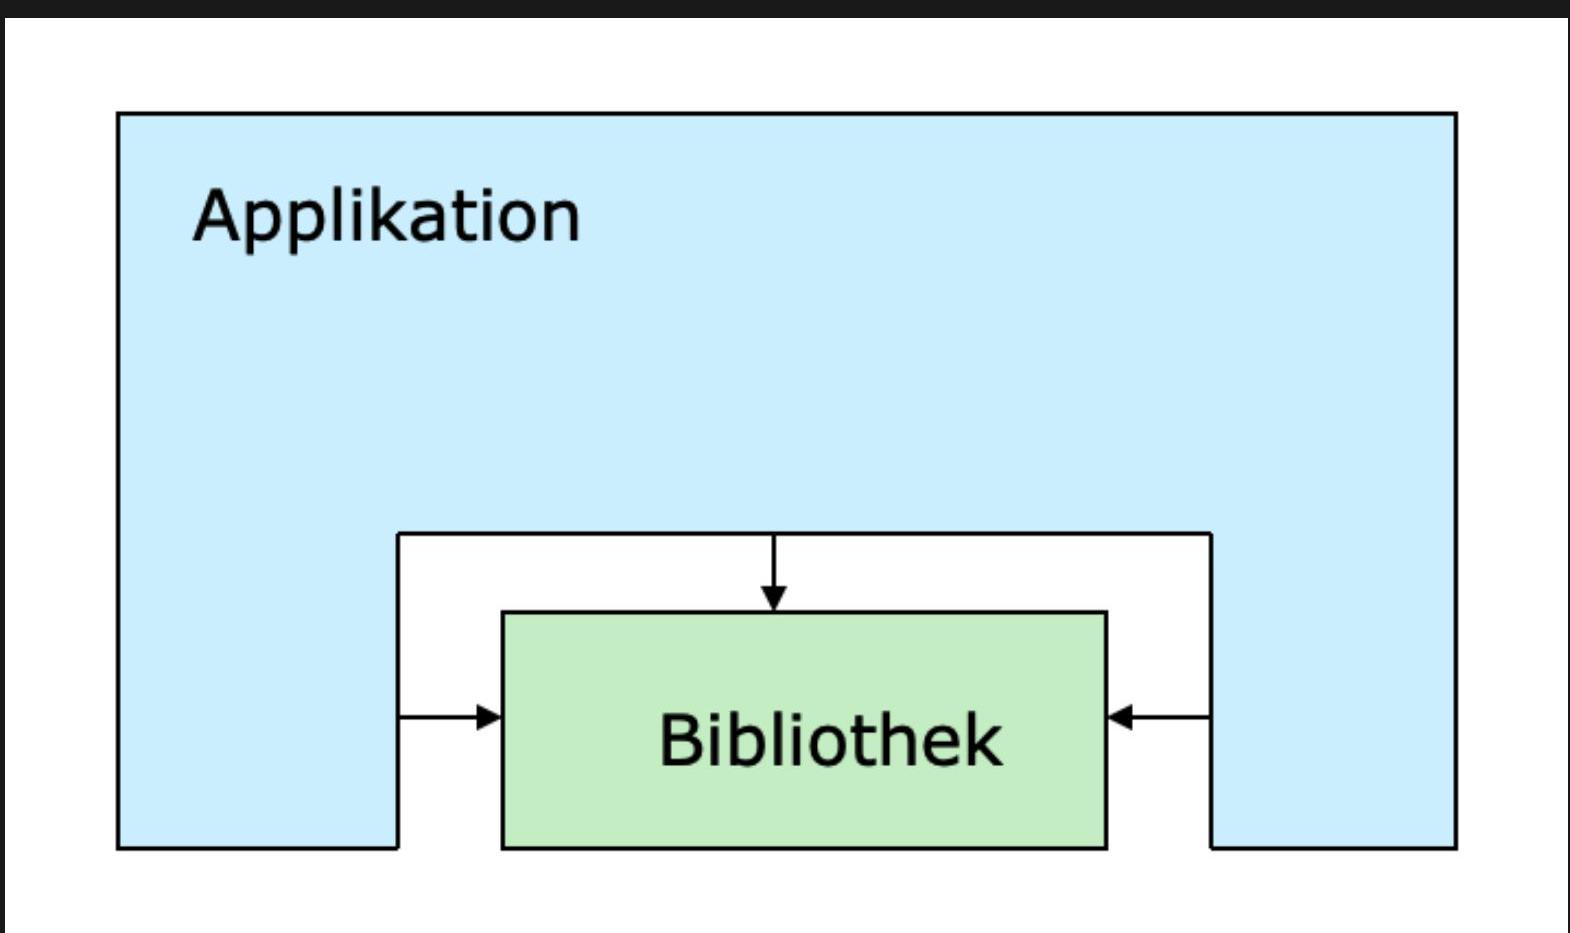
\includegraphics[width=\linewidth]{images/2025_01_02_22162ee5453ad0230328g-04}
\end{itemize}

\section*{FRAMEWORK}
\begin{itemize}
  \item Rahmen für die Anwendung
  \item Kontrolle liegt beim Framework
  \item Hollywood-Prinzip: „don't call us, we'll call you"\\
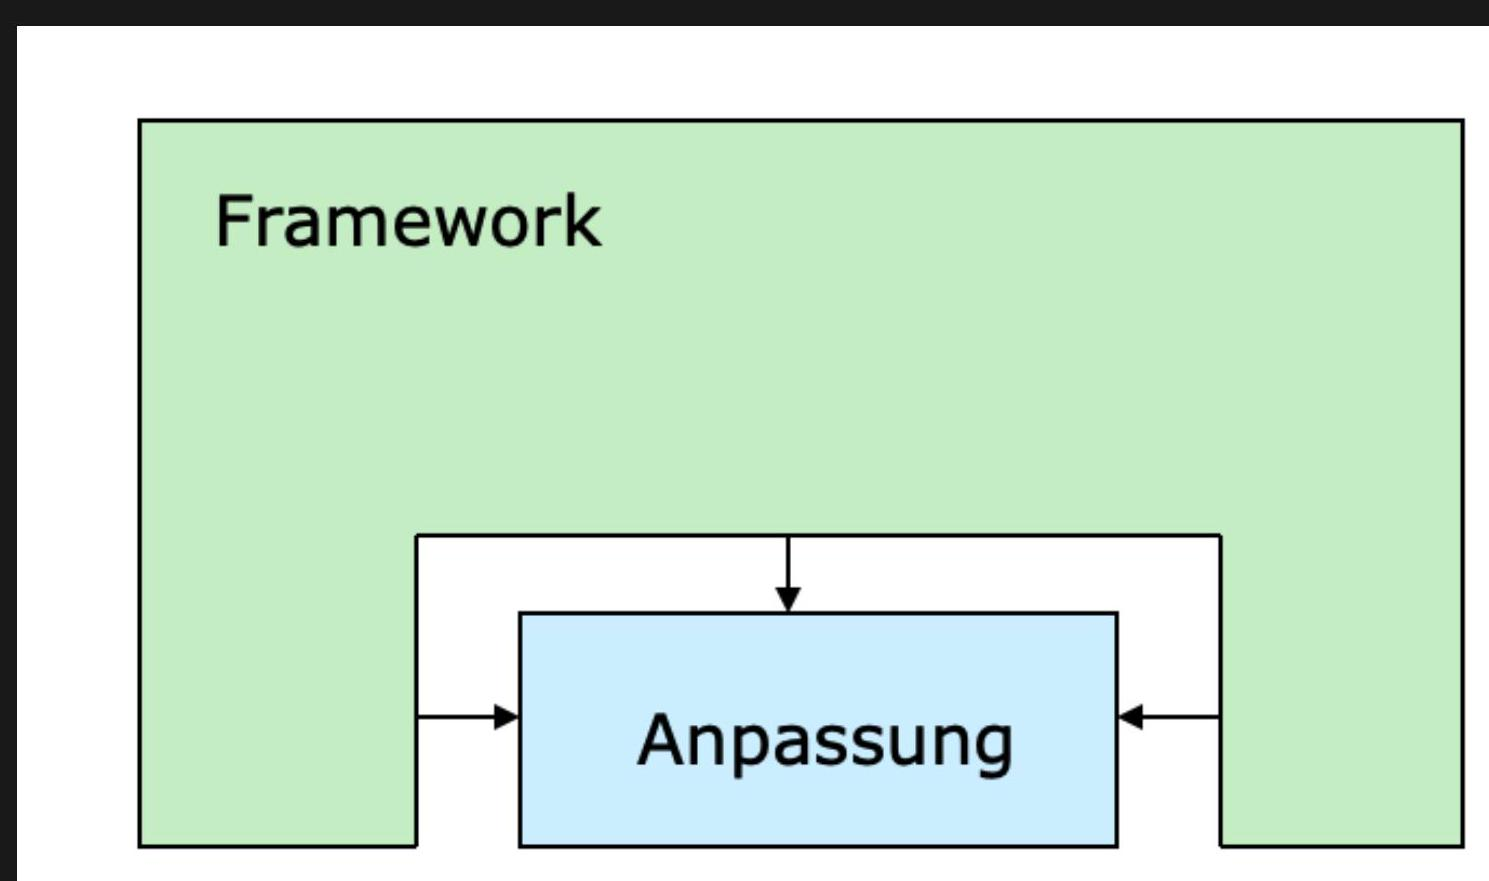
\includegraphics[width=\linewidth]{images/2025_01_02_22162ee5453ad0230328g-05}
\end{itemize}

\section*{ANSÄTZE IM LAUF DER ZEIT}
\begin{itemize}
  \item Statische Webseiten
  \item Inhalte dynamisch generiert (CGI z.B. Shell Scripts, Perl)
  \item Serverseitig eingebettete Scriptsprachen (PHP)
  \item Client Scripting oder Applets (JavaScript, Java Applets, Flash)
  \item Enterprise Application Server (Java, Java EE)
  \item MVC Server-Applikationen (Rails, Django)
  \item JavaScript Server (Node.js)
  \item Single Page Applikationen (SPAs)
\end{itemize}

\section*{SERVERSEITE}
\begin{itemize}
  \item Verschiedene Technologien möglich
  \item Zahlreiche Bibliotheken und Frameworks
  \item Verschiedene Architekturmuster
  \item Häufig: Model-View-Controller (MVC)
  \item Beispiel: Ruby on Rails
\end{itemize}

\section*{MODEL-VIEW-CONTROLLER (MVC)}
Models

\begin{itemize}
  \item repräsentieren anwendungsspezifisches Wissen und Daten
  \item ähnlich Klassen: User, Photo, Todo, Note
  \item können Observer über Zustandsänderungen informieren
\end{itemize}

\section*{Views}
\begin{itemize}
  \item bilden die Benutzerschnittstelle (z.B. HTML/CSS)
  \item können Models überwachen, kommunizieren aber normalerweise nicht direkt mit innen
\end{itemize}

\section*{Controllers}
\begin{itemize}
  \item verarbeiten Eingaben (z.B. Clicks) und aktualisieren Models
\end{itemize}

\section*{RUBY ON RAILS}
\begin{itemize}
  \item Serverseitiges Framework, basierend auf MVC
  \item Programmiersprache: Ruby\\
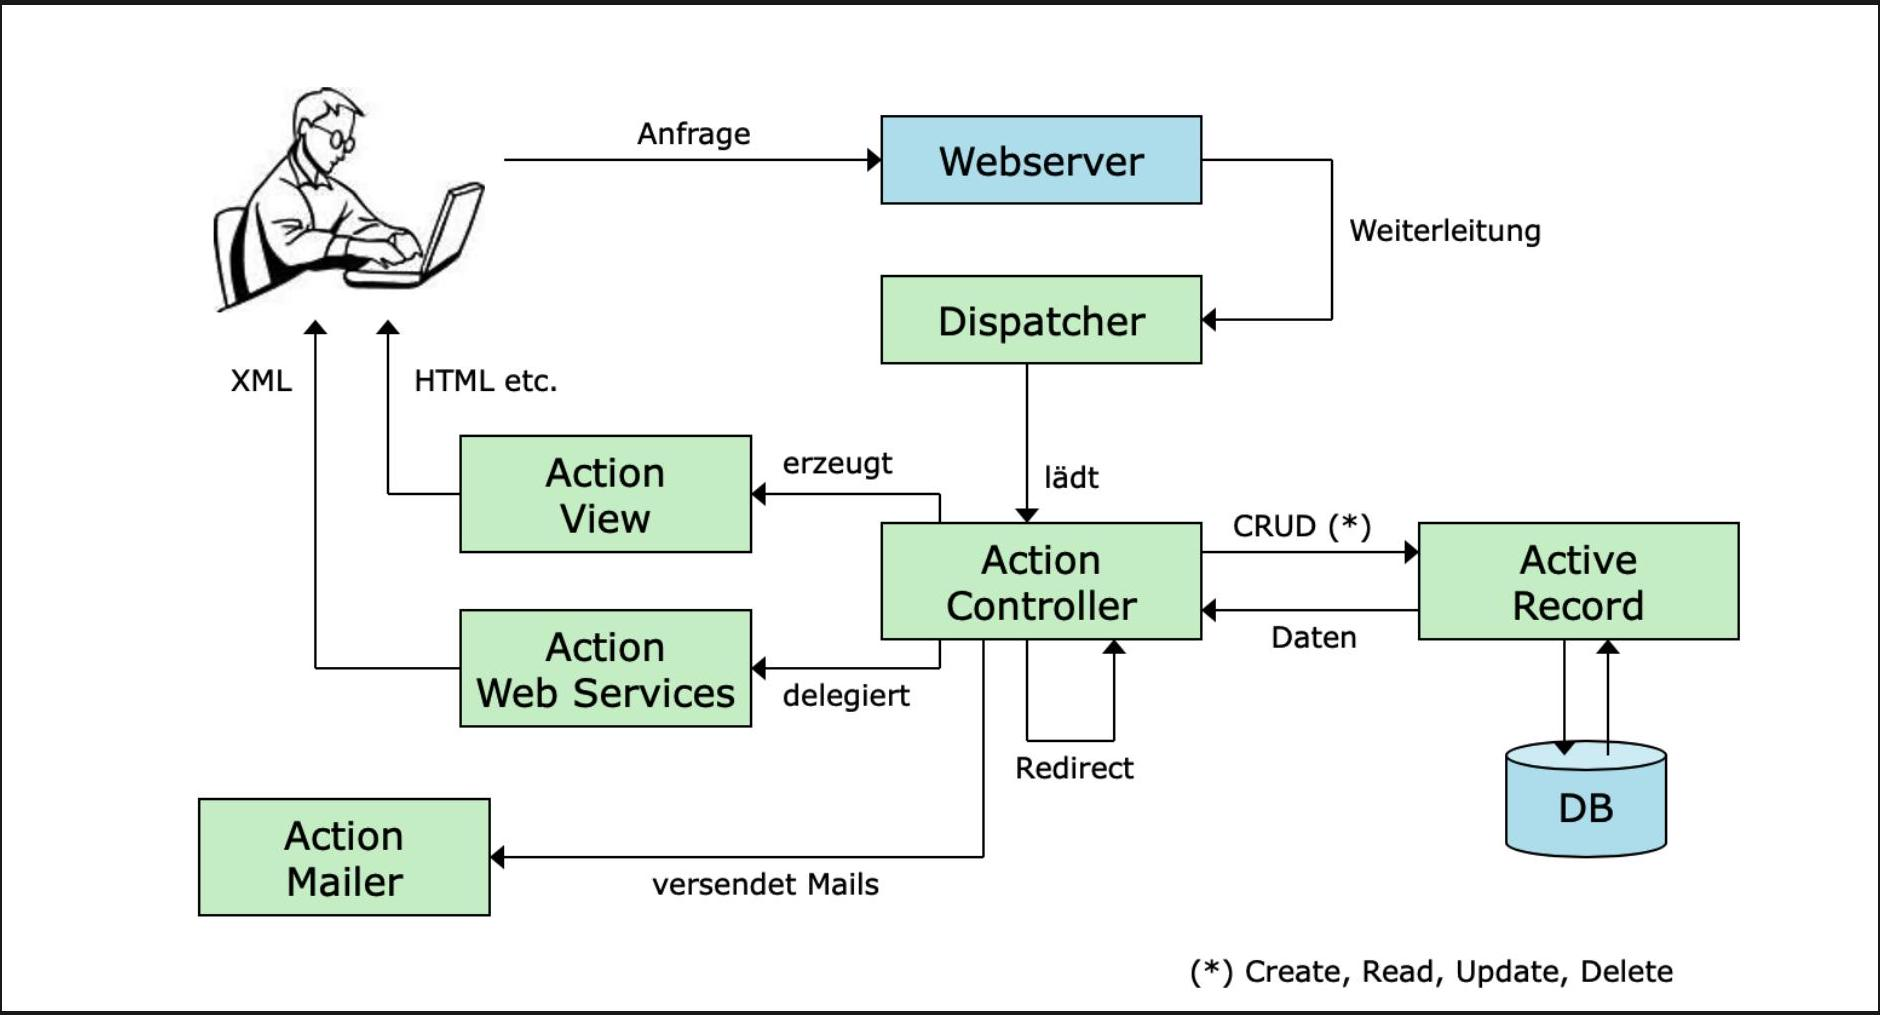
\includegraphics[width=\linewidth]{images/2025_01_02_22162ee5453ad0230328g-09}
\end{itemize}

\section*{Convention over Configuration}
\href{https://rubyonrails.org}{https://rubyonrails.org}

\section*{FOKUS AUF DIE CLIENT-SEITE}
\begin{itemize}
  \item Programmlogik Richtung Client verschoben
  \item Zunehmend komplexe User Interfaces
  \item Asynchrone Serveranfragen, z.B. mit Fetch
  \item Gute Architektur der Client-App wesentlich
  \item Diverse Frameworks und Bibliotheken zu diesem Zweck
\end{itemize}

\section*{SINGLE PAGE APPS (SPAs)}
\begin{itemize}
  \item Neuladen von Seiten vermeiden
  \item Inhalte dynamisch nachgeladen (Ajax, REST)
  \item Kommunikation mit Server im Hintergrund
  \item Ul reagiert schneller (Usability)
\end{itemize}

\section*{ÜBERSICHT}
\begin{itemize}
  \item Frameworks und Bibliotheken
  \item DOM-Scripting und Abstraktionen
  \item JSX und SJDON
  \item Eigene Bibliothek: SuiWeb
\end{itemize}

\section*{DOM-SCRIPTING}
\begin{itemize}
  \item Zahlreiche Funktionen und Attribute verfügbar
  \item Programme werden schnell unübersichtlich
  \item Gesucht: geeignete Abstraktionen
\end{itemize}

\section*{AUFGABE}
\begin{itemize}
  \item Zum Vergleich der verschiedenen Ansätze
  \item Liste aus einem Array erzeugen
\end{itemize}

\begin{verbatim}
/* gegeben: */
let data = ["Maria", "Hans", "Eva", "Peter"]
<!-- DOM-Struktur entsprechend folgendem Markup aufzubauen: -->
<ul>
    <li>Maria</li>
    <li>Hans</li>
    <li>Eva</li>
    <li>Peter</li>
</ul>
\end{verbatim}

\section*{DOM-SCRIPTING}
\begin{verbatim}
function List (data) {
    let node = document.createElement("ul")
    for (let item of data) {
        let elem = document.createElement("li")
        let elemText = document.createTextNode(item)
        elem.appendChild(elemText)
        node.appendChild(elem)
    }
    return node
}
\end{verbatim}

\begin{itemize}
  \item Erste Abstraktion: Listen-Komponente
  \item Basierend auf DOM-Funktionen
\end{itemize}

\section*{DOM-SCRIPTING}
\begin{verbatim}
function init () {
    let app = document.querySelector(".app")
    let data = ["Maria", "Hans", "Eva", "Peter"]
    render(List(data), app)
}
function render (tree, elem) {
    while (elem.firstChild) { elem.removeChild(elem.firstChild) }
    elem.appendChild(tree)
}
\end{verbatim}

\section*{DOM-SCRIPTING VERBESSERT}
\begin{verbatim}
function elt (type, attrs, ...children) {
    let node = document.createElement(type)
    Object.keys(attrs).forEach(key => {
        node.setAttribute(key, attrs[key])
    })
    for (let child of children) {
        if (typeof child != "string") node.appendChild(child)
        else node.appendChild(document.createTextNode(child))
    }
    return node
}
\end{verbatim}

\section*{DOM-SCRIPTING VERBESSERT}
\begin{itemize}
  \item Damit vereinfachte List-Komponente möglich
  \item DOM-Funktionen in einer Funktion elt gekappselt
\end{itemize}

\begin{verbatim}
function List (data) {
    return elt("ul", {}, ...data.map(item => elt("li", {}, item)))
}
\end{verbatim}

\section*{JQUERY}
\begin{verbatim}
function List (data) {
    return $("<ul>").append(...data.map(item => $("<li>").text(item)))
}
function render (tree, elem) {
    while (elem.firstChild) { elem.removeChild(elem.firstChild) }
    $(elem).append(tree)
}
\end{verbatim}

\begin{itemize}
  \item List gibt nun ein jQuery-Objekt zurück
  \item Daher ist eine kleine Anpassung an render erforderlich
\end{itemize}

\section*{WEB COMPONENTS}
\begin{itemize}
  \item Möglichkeit, eigene Elemente zu definieren
  \item Implementiert mit HTML, CSS und JavaScript
  \item Implementierung im Shadow DOM verstecken
\end{itemize}

\begin{verbatim}
<custom-progress-bar class="size">
<custom-progress-bar value="25">
<script>
    document.querySelector('.size').progress = 75;

\section*{REACT.JS}
\end{verbatim}

const List = (\{data\}) => (\\
\\
\{ data.map(item => (\{item\})) \}\\
\\
)\\
const root = createRoot(document.getElementById('app'))\\
root.render(\\[0pt]
<List data=\{["Maria", "Hans", "Eva", "Peter"]\} />\\
)

\begin{verbatim}
- XML-Syntax in JavaScript: JSX
- Muss zu JavaScript übersetzt werden
- https://reactjs.org

\section*{VUE.JS}
\end{verbatim}

\begin{verbatim}
https://vuejs.org
\end{verbatim}

var app4 = new Vue(\{\\
el: '\#app',\\
data: \{\\
items: [\\
\{ text: 'Learn JavaScript' \},\\
\{ text: 'Learn Vue' \},\\
\{ text: 'Build something awesome' \}\\[0pt]
]\\
\}\\
\})

\begin{verbatim}

\section*{ÜBERSICHT}
- Frameworks und Bibliotheken
- DOM-Scripting und Abstraktionen
- JSX und SJDON
- Eigene Bibliothek: SuiWeb

\section*{EIGENE BIBLIOTHEK}
- Ziel: eigene kleine Bibliothek entwickeln
- Ideen von React.js als Grundlage
- In dieser und den folgenden Lektionen schrittweise aufgebaut
- Wir nennen es:

\author{
SuiWeb \\ Simple User Interface Toolkit for Web Exercises
}

\section*{EIGENE BIBLIOTHEK: MERKMALE}
![](https://cdn.mathpix.com/cropped/2025_01_02_22162ee5453ad0230328g-25.jpg?height=1024&width=891&top_left_y=856&top_left_x=243)
- Komponentenbasiert
- Also: User Interface aus Komponenten zusammengesetzt
- Zum Beispiel:

Komponente ArticleList

\section*{EIGENE BIBLIOTHEK: MERKMALE}
![](https://cdn.mathpix.com/cropped/2025_01_02_22162ee5453ad0230328g-26.jpg?height=1101&width=704&top_left_y=813&top_left_x=241)
- Datengesteuert
- Input: Daten der Applikation
- Output: DOM-Struktur für Browser

\section*{(data) =>}
![](https://cdn.mathpix.com/cropped/2025_01_02_22162ee5453ad0230328g-27.jpg?height=547&width=838&top_left_y=951&top_left_x=1901)

\section*{NOTATION FÜR KOMPONENTEN}
- Gesucht: Notation zum Beschreiben von Komponenten
- Ziel: möglichst deklarativ
- Also nicht: imperativen JavaScript- oder jQuery-Code, der DOM manipuliert
- Verschiedene Möglichkeiten, z.B.
- JSX: in React.js verwendet
- SJDON: eigene Notation
\end{verbatim}

JSX\\
const Hello = () => (\\
Hello World\\
)

\begin{verbatim}
- Von React-Komponenten verwendete Syntax
- Komponente beschreibt DOM-Struktur mittels JSX
- HTML-Markup gemischt mit eigenen Tags
- JSX = JavaScript XML
(oder: JavaScript Syntax Extension?)

\section*{JSX INS DOM ABBILDEN}
\end{verbatim}

const domNode = document.getElementById('app')\\
const root = createRoot(domNode)\\
root.render()

\begin{verbatim}
- Root zum Rendern der Komponente anlegen
- Methode render aufrufen mit Code der gerendert werden soll

\section*{JSX}
- Problem: das ist kein JavaScript-Code
- Sondern: JavaScript-Code mit XML-Teilen
- Muss erst in JavaScript-Code übersetzt werden (Transpiler)
- Browser erhält pures JavaScript
![](https://cdn.mathpix.com/cropped/2025_01_02_22162ee5453ad0230328g-31.jpg?height=780&width=2082&top_left_y=1399&top_left_x=222)

\section*{JSX: HTML-ELEMENTE}
- HTML-Elemente als vordefinierte Komponenten
- Somit können beliebige HTML-Elemente in Komponenten verwendet werden
root.render(A Header)
\end{verbatim}



\begin{verbatim}

\section*{JSX: HTML-ELEMENTE}
- HTML-Tags in Kleinbuchstaben
- Eigene Komponenten mit grossen Anfangsbuchstaben
- HTML-Elemente können die üblichen Attribute haben
- Wenige Ausnahmen, z.B.:
class-Attribut heisst className in JSX

\section*{JSX: KOMPONENTEN}
\end{verbatim}

1 const MyComponent = () => (\\

My Component
Content in my component...
\\
)\\
root.render(\\
\\
10 )

\begin{verbatim}

\section*{JSX: KOMPONENTEN}
\end{verbatim}

const List = (\{data\}) => (\\
\\
\{ data.map(item => (\{item\})) \}\\
\\
)\\
root.render(\\[0pt]
<List data=\{["Maria", "Hans", "Eva", "Peter"]\} />\\
)

\begin{verbatim}
- JavaScript in JSX in \{... \}

\section*{JSX: KOMPONENTEN}
- Funktionen, welche JSX-Code zurückgeben
- Neue Komponente kann dann als Tag im JSX benutzt werden
- Üblicherweise werden Komponenten in eigenen Modulen implementiert und bei Bedarf importiert

\section*{SJDON}
- Alternative zu JSX, eigene Notation
- SJDON - Simple JavaScript DOM Notation
- Bezeichnung aus einer Semesterendprüfung in WWD (WebPublishing und Webdesign, G. Burkert, 2011 an der ZHAW)
4. JavaScript-Datenstrukturen, JSON, PHP (12 Punkte)

In einer Ajax-Anwendung soll HTML-Code in einfachen JavaScript-Datenstrukturen aufgebaut und manipuliert werden. Diese können dann im JSON-Format an den Server übertragen und zum Beispiel in einer Datenbank gespeichert werden. Schliesslich lässt sich aus den Strukturen auf relativ einfache Weise wieder HTML-Code generieren.

Die Notation - nennen wir sie SJDON (Simple JavaScript DOM Notation) - sei wie folgt definiert:

Die Notation - nennen wir sie SJDON (Simple JavaScript DOM Notation) - sei wie folgt definiert:
- Ein Textknoten ist einfach der String mit dem Text.
- Ein Elementknoten ist ein Array, das als erstes den Elementnamen als String enthält und anschliessend die Kindelemente (Text- oder Elementknoten, in der gewünschten Reihenfolge) und Attributbeschreibungen für den Elementknoten.
- Attributbeschreibungen sind Objekte deren Attribute und Werte direkt den Attributen und Werten des HTML-Elements entsprechen. Alle Attribute des Elements können in einem Objekt zusammengefasst oder auf mehrere Objekte verteilt werden.
![](https://cdn.mathpix.com/cropped/2025_01_02_22162ee5453ad0230328g-38.jpg?height=919&width=2313&top_left_y=1119&top_left_x=647)

\section*{VERGLEICH}
\end{verbatim}

/* JSX \textit
%{/\\
const element = (\\
Hello World
from SuiWeb
)\\
%/} SJDON */\\
const element =\\[0pt]
["div", \{style: "background:salmon"\},\\[0pt]
["h1", "Hello World"],\\[0pt]
["h2", \{style: "text-align:right"\}, "from SuiWeb"] ]

\begin{verbatim}

\section*{ELEMENTE}
- Ein Element wird als Array repräsentiert
- Das erste Element ist der Elementknoten
- String: DOM-Knoten mit diesem Typ
- Funktion: Selbst definierte Komponente
\end{verbatim}

["br"] /* br-Element \textit{/\\[0pt]
["ul", ["li", "eins"], ["li", "zwei"]] /} Liste mit zwei Items \textit{/\\[0pt]
[App, \{name: "SuiWeb"\}] /} Funktionskomponente */

\begin{verbatim}

\section*{ATTRIBUTE}
- Als Objekte repräsentiert
- Irgendwo im Array (ausser ganz vorne)
- Mehrere solcher Objekte werden zusammengeführt
\end{verbatim}

/* mit style-Attribut, Reihenfolge egal */\\[0pt]
["p", \{style: "text-align:right"\}, "Hello world"]\\[0pt]
["p", "Hello world", \{style: "text-align:right"\}]

\begin{verbatim}

\section*{FUNKTIONEN}
- Funktion liefert SJDON-Ausdruck
- Kein \{ . . . \} für JavaScript wie in JSX nötig
\end{verbatim}

const App = (\{name\}) =>\\[0pt]
["h1", "Hi ", name]\\
const element =\\[0pt]
[App, \{name: "SuiWeb"\}]

\begin{verbatim}

\section*{BEISPIEL: LISTENKOMPONENTE}
\end{verbatim}

const MyList = (\{items\}) =>\\[0pt]
["ul", ...items.map(item => ["li", item]) ]\\
const element =\\[0pt]
[MyList, \{items: ["milk", "bread", "sugar"]\}]

\begin{verbatim}
- JavaScript-Ausdruck generiert Kind-Elemente für ul
- Kein Problem, JavaScript-Ausdrücke einzufügen SJDON is pure JavaScript ;)

\section*{ÜBERSICHT}
- Frameworks und Bibliotheken
- DOM-Scripting und Abstraktionen
- JSX und SJDON
- Eigene Bibliothek: SuiWeb

\section*{ZIEL}
- Bau einer kleinen Web-Bibliothek
- Ausgerichtet an den Ideen von React
- Komponenten in JSX oder SJDON

\author{
Motto: \\ Keep it simple
}

\section*{SuiWeb}
- Simple User Interface Toolkit for Web Exercises
- Kein Mega-Framework
- Keine "full-stack"-Lösung
- Daten steuern Ausgabe der Komponenten
- Komponenten können einen Zustand haben

\section*{KEIN TWO-WAY-BINDING}
![](https://cdn.mathpix.com/cropped/2025_01_02_22162ee5453ad0230328g-47.jpg?height=365&width=1843&top_left_y=750&top_left_x=408)
- Ul-Elemente nicht bidirektional mit Model-Daten verbunden
- Daten werden verwendet, um View zu generieren
- Benutzerinteraktionen bewirken ggf. Anpassungen am Model
- Dann wird die View erneut aus den Daten generiert

\section*{AUSBLICK}
- Schrittweiser Aufbau von SuiWeb
- Beispiele im Praktikum

Wichtiger Hinweis: React.js ist ein bekanntes und verbreitetes Framework und JSX eine bekannte Notation. SJDON und SuiWeb sind eigene Entwicklungen und ausserhalb WBE unbekannt...


\subsection{UI Implementierung}

\begin{itemize}
    \item Interne Repräsentation und das DOM
    \item Komponenten und Properties
    \item Darstellung von Komponenten
    \item Defaults und weitere Beispiele
  \end{itemize}
  
  \section*{ÜBERSICHT}
  \begin{itemize}
    \item Interne Repräsentation und das DOM
    \item Komponenten und Properties
    \item Darstellung von Komponenten
    \item Defaults und weitere Beispiele
  \end{itemize}
  
  \section*{RÜCKBLICK}
  \begin{itemize}
    \item Ziel: eigene kleine Bibliothek entwickeln
    \item Komponentenbasiert und datengesteuert
    \item An Ideen von React.js und ähnlicher Systeme orientiert
    \item Motto: „Keep it simple!"
    \item Bezeichnung:
  \end{itemize}
  
  \section*{SuiWeb}
  Simple User Interface Toolkit for Web Exercises
  
  \section*{RÜCKBLICK}
  \begin{itemize}
    \item Notation für den Aufbau der Komponenten
    \item JSX: in React.js verwendet
    \item SJDON: eigene Notation
    \item SuiWeb soll beide Varianten unterstützen
  \end{itemize}
  
  \begin{verbatim}
  // jsx
  const element = (<h1 title="foo">Hello</h1>)
  // sjdon
  const element = ["h1", {title: "foo"}, "Hello"]
  \end{verbatim}
  
  \section*{ANSTEHENDE AUFGABEN}
  \begin{itemize}
    \item Interne Repräsentation der Komponenten
    \item Konvertierung von JSX und SJDON in diese Repräsentation
    \item Abbildung interne Repräsentation ins DOM
    \item Daten steuern Komponenten: Properties
    \item Hierarchie von Komponenten
    \item Komponenten mit Zustand
  \end{itemize}
  
  Anregungen und Code-Ausschnitte aus:\\
  Rodrigo Pombo: Build your own React\\
  \href{https://pomb.us/build-your-own-react/}{https://pomb.us/build-your-own-react/}\\
  Zachary Lee: Build Your Own React.js in 400 Lines of Code \href{https://webdeveloper.beehiiv.com/p/build-react-400-lines-code}{https://webdeveloper.beehiiv.com/p/build-react-400-lines-code}
  
  \section*{AUSGANGSPUNKT}
  \begin{verbatim}
  // jsx
  /** @jsx createElement */
  const element = (<h1 title="foo">Hello</h1>)
  // jsx babel output (React < 17)
  const element = createElement(
      "h1",
      { title: "foo" },
      "Hello"
  )
  // sjdon
  const element = ["h1", {title: "foo"}, "Hello"]
  \end{verbatim}
  
  \section*{INTERNE REPRÄSENTATION}
  \begin{verbatim}
  // jsx babel output
  const element = createElement(
      "h1",
      { title: "foo" },
      "Hello"
  )
  \end{verbatim}
  
  \begin{verbatim}
  // internal representation
  const element = {
      type: "h1",
      props: {
          title: "foo",
          children: ["Hello"],
      },
  }
  \end{verbatim}
  
  \section*{INTERNE REPRÄSENTATION}
  \begin{verbatim}
  {
      type: "h1",
      props: {
          title: "foo",
          children: ["Hello"], /* noch anzupassen */
      },
  }
  \end{verbatim}
  
  \begin{itemize}
    \item Element: Objekt mit zwei Attributen, type und props
    \item type: Name des Elements ("body", "h1", ...)
    \item props: Attribute des Elements
    \item props.children: Kindelemente (Array)
  \end{itemize}
  
  \section*{TEXT-ELEMENT}
  \begin{verbatim}
  {
      type: "TEXT_ELEMENT",
      props: {
          nodeValue: "Hello",
          children: [],
      },
  }
  \end{verbatim}
  
  \begin{itemize}
    \item Aufbau analog zu anderen Elementen
    \item Spezieller Typ: "TEXT\_eLEMENT"
  \end{itemize}
  
  \section*{VERSCHACHTELTE ELEMENTE}
  \begin{center}
  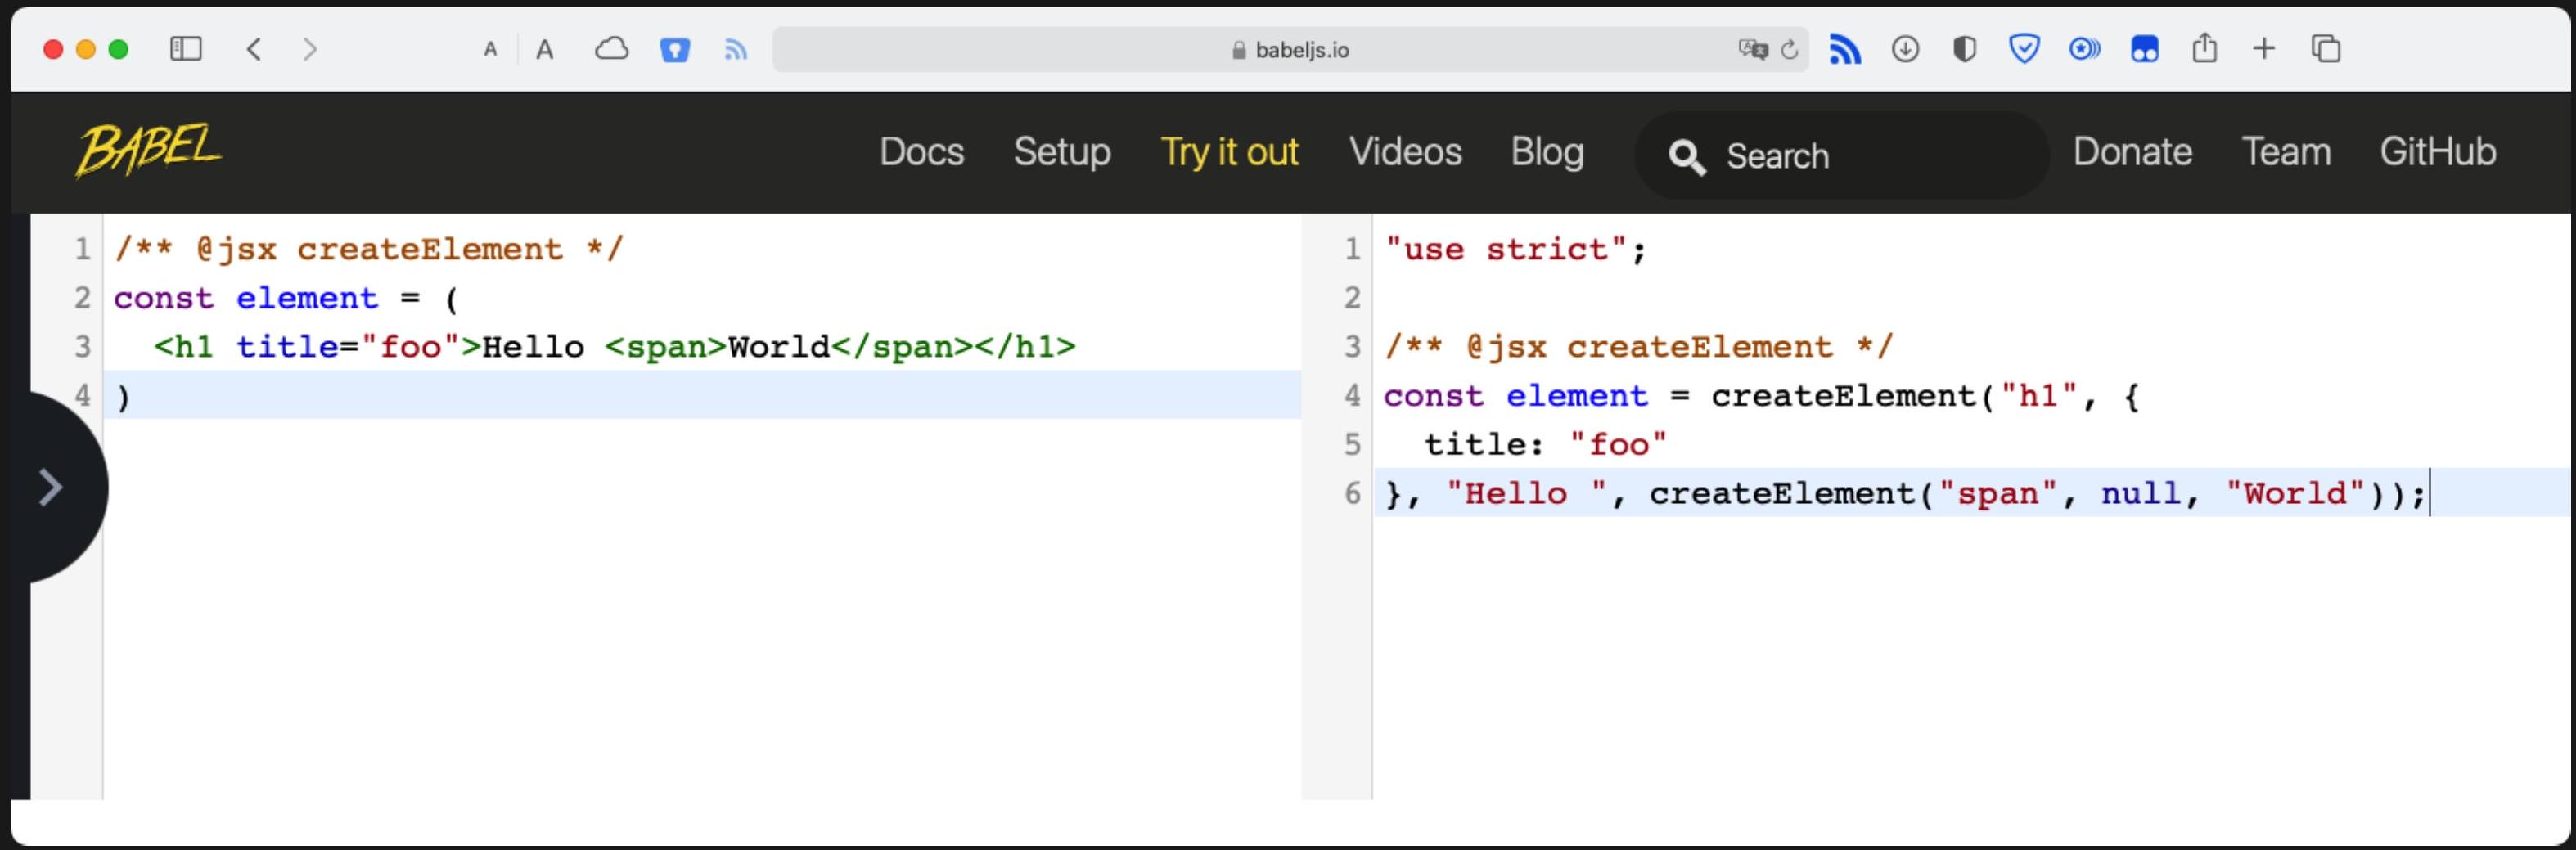
\includegraphics[width=\linewidth]{images/2025_01_02_254b5e4c52d090c313e1g-11}
  \end{center}
  
  \begin{itemize}
    \item Mehrere Kindelemente: ab drittem Argument von createElement
    \item Verschachtelte Elemente: rekursive Aufrufe von createElement
  \end{itemize}
  
  \section*{KONVERTIERUNG VON JSX}
  \begin{verbatim}
  function createElement (type, props,
                                  ...children) {
      return {
          type,
          props: {
              ...props,
              children: children.map(child =>
                  typeof child === "object"
                      ? child
                  : createTextElement(child)
              ),
      },
      }
  }
  \end{verbatim}
  
  \begin{verbatim}
  function createTextElement (text) {
      return {
          type: "TEXT_ELEMENT",
          props: {
              nodeValue: text,
              children: [],
          },
      }
  }
  \end{verbatim}
  
  \section*{CREATEELEMENT: BEISPIEL}
  \begin{verbatim}
  // <div>Hello<br></div>
  createElement("div", null, "Hello", createElement("br", null))
  // returns
  {
      type: 'div',
      props: {
          children: [
              {
                  type: 'TEXT_ELEMENT',
                      props: { nodeValue: 'Hello', children: [] }
              },
              { type: 'br', props: { children: [] } }
          ]
      }
  }
  \end{verbatim}
  
  \section*{KONVERTIERUNG VON SJDON}
  \begin{verbatim}
  function parseSJDON ([type, ...rest]) {
      const isObj = (obj) => typeof(obj)==='object' && !Array.isArray(obj)
      const children = rest.filter(item => !isObj(item))
      return createElement(type,
          Object.assign({}, ...rest.filter(isObj)),
          ...children.map(ch => Array.isArray(ch) ? parseSJDON(ch) : ch)
      )
  }
  \end{verbatim}
  
  \begin{itemize}
    \item Abbildung auf createElement-Funktion
    \item Attribute in einem Objekt zusammengeführt
    \item Kindelemente bei Bedarf (Array) ebenfalls geparst
  \end{itemize}
  
  \section*{ZWISCHENSTAND}
  \begin{itemize}
    \item Einheitliche Repräsentation für Elemente unabhängig von der ursprünglichen Syntax (JSX or SJDON)
    \item Baumstruktur von Elementen
    \item Text-Elemente mit leerem Array children
    \item DOM-Fragment im Speicher repräsentiert (virtuelles DOM?)
  \end{itemize}
  
  Zu tun:
  
  \begin{itemize}
    \item Abbildung der Baumstruktur ins DOM
  \end{itemize}
  
  \section*{RENDER TO DOM}
  \begin{verbatim}
  function render (element, container) {
      /* create DOM node */
      const dom =
          element.type == "TEXT_ELEMENT"
              ? document.createTextNode("")
              : document.createElement(element.type)
      /* assign the element props */
      const isProperty = key => key !== "children"
      Object.keys(element.props)
          .filter(isProperty)
          .forEach(name => { dom[name] = element.props[name] })
      /* render children */
      element.props.children.forEach(child => render(child, dom))
      /* add node to container */
      container.appendChild(dom)
  }
  \end{verbatim}
  
  \section*{HTML-ELEMENTE}
  \begin{itemize}
    \item Komponenten können HTML-Elemente verwenden
    \item Tagnamen in Kleinbuchstaben
    \item Gross-/Kleinschreibung ist relevant
    \item Übliche Attribute für HTML-Elemente möglich
    \item Wenig Ausnahmen: className statt class
  \end{itemize}
  
  \section*{BEISPIEL}
  \begin{center}
  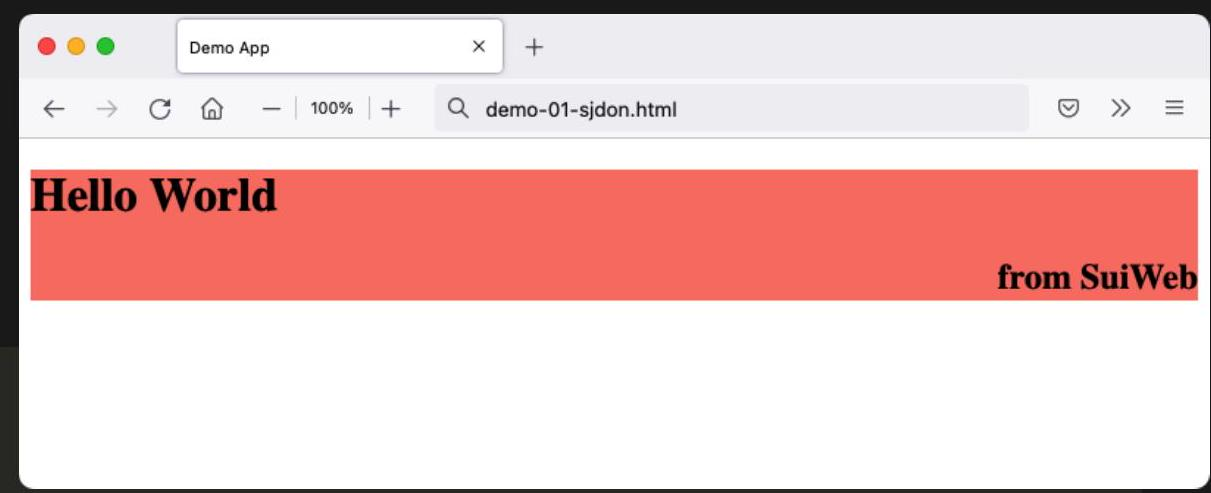
\includegraphics[width=\linewidth]{images/2025_01_02_254b5e4c52d090c313e1g-18}
  \end{center}
  
  \begin{verbatim}
  import { render } from "./lib/suiweb-1.1.js"
  const element =
      ["div", {style: "background:salmon"},
          ["h1", "Hello World"],
          ["h2", {style: "text-align:right"}, "from SuiWeb"] ]
  const container = document.getElementById("root")
  render(element, container)
  \end{verbatim}
  
  \section*{ZWISCHENSTAND}
  \begin{itemize}
    \item Interne Struktur aufbauen
    \item Ins DOM rendern
  \end{itemize}
  
  
  
  \section*{ÜBERSICHT}
  \begin{itemize}
    \item Interne Repräsentation und das DOM
    \item Komponenten und Properties
    \item Darstellung von Komponenten
    \item Defaults und weitere Beispiele
  \end{itemize}
  
  \section*{FUNKTIONSKOMPONENTEN}
  \begin{verbatim}
  1 const App = (props) =>
      ["h1", "Hi ", props.name]
  4 const element =
  5 [App, {name: "foo"}]
  \end{verbatim}
  
  \begin{itemize}
    \item App ist eine Funktionskomponente
    \item Die zugehörige Repräsentation erzeugt keinen DOM-Knoten
    \item Ergebnis des Aufrufs liefert auszugebende Struktur
    \item Konvention: eigene Komponenten mit grossen Anfangsbuchstaben
  \end{itemize}
  
  \section*{PROBLEM}
  \begin{itemize}
    \item Komponenten in JSX retournieren mittels createElement erzeugte interne Strukturen
    \item Unter SJDON liefern sie allerdings SJDON-Code, der nach Aufruf der Komponente noch geparst werden muss
    \item Abhilfe: SJDON-Komponenten erhalten ein Attribut sjdon, welches die Konvertierung (parseSJDON ) ergänzt
    \item Dieses Attribut lässt sich mit einer kleinen Hilfsfunktion anbringen
  \end{itemize}
  
  \section*{SJDON-KONVERTIERUNG ERWEITERT}
  \begin{verbatim}
  function useSJDON (...funcs) {
      for (let f of funcs) {
          const fres = (...args) => parseSJDON(f(...args))
          f.sjdon = fres
      }
  }
  \end{verbatim}
  
  \begin{itemize}
    \item Kann für mehrere Komponentenfunktionen aufgerufen werden, indem sie als Argumente übergeben werden
    \item Diese werden um das sjdon-Attribut ergänzt
  \end{itemize}
  
  \section*{FUNKTIONSKOMPONENTEN}
  \begin{itemize}
    \item Funktion wird mit props-Objekt aufgerufen
    \item Ergebnis ggf. als SJDON geparst
  \end{itemize}
  
  \begin{verbatim}
  switch (typeof type)
      case 'function': {
          let children
          if (typeof(type.sjdon) === 'function') {
              children = type.sjdon(props)
          } else {
              children = type(props)
          }
          reconcileChildren(...)
          break
      }
  }
  \end{verbatim}
  
  \section*{BEISPIEL}
  \begin{verbatim}
  const App = (props) =>
      ["h1", {style: "background: mediumaquamarine"}, "Hi ", props.name]
  const element =
      [App, {name: "SuiWeb"}]
  // notify SuiWeb that the App component returns SJDON
  useSJDON(App)
  const container = document.getElementById ©\bullet. Domonop
  render(element, container)
  demo-02-jsx.html demo-02-sjdon.html
  \end{verbatim}
  
  \begin{center}
  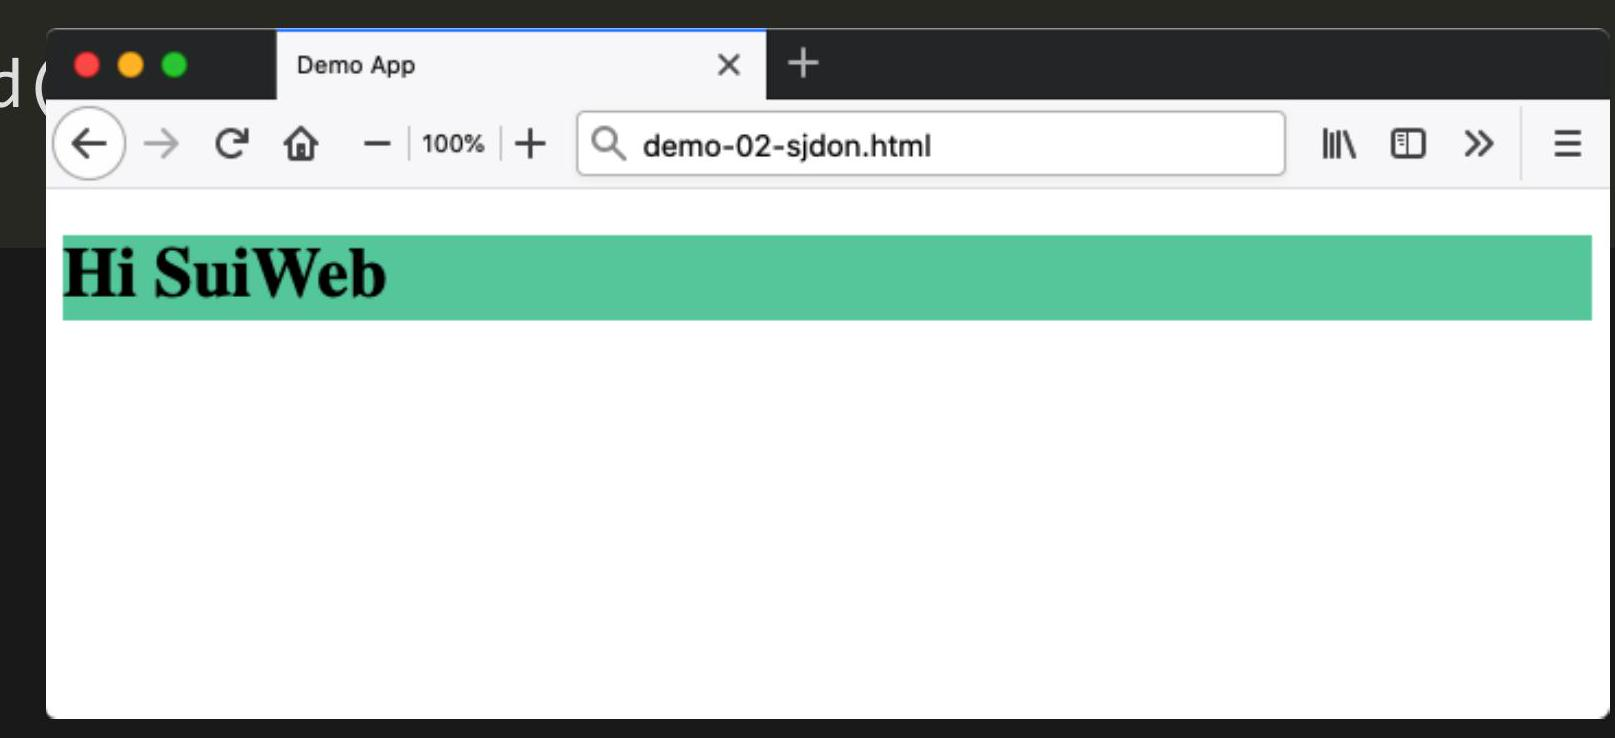
\includegraphics[width=\linewidth]{images/2025_01_02_254b5e4c52d090c313e1g-25}
  \end{center}
  
  \section*{WERTE STEUERN UI-AUFBAU}
  \begin{verbatim}
  const App = () => {
      const enabled = false
      const text = 'A Button'
      const placeholder = 'input value...'
      const size = 50
      return (
          ["section",
              ["button", {disabled: !enabled}, text],
              ["input", {placeholder, size, autofocus: true}] ]
      )
  }
  \end{verbatim}
  
  demo-03-values
  
  \section*{ARRAY ALS LISTE AUSGEBEN}
  \begin{verbatim}
  const List = ({items}) =>
      ["ul", ...items.map((item) => ["li", item]) ]
  const element =
      [List, {items: ["milk", "bread", "sugar"]}]
  useSJDON(List)
  \end{verbatim}
  
  \begin{itemize}
    \item Die props werden als Argument übergeben
    \item Hier interessiert nur das Attribut items\\
  demo-04-liste
  \end{itemize}
  
  \section*{OBJEKT ALS TABELLE}
  \begin{verbatim}
  const ObjTable = ({obj}) =>
      ["table", {style},
          ...Object.keys(obj).map((key) =>
          ["tr", ["td", key], ["td", obj[key]]])]
  const style = {
      width: "8em",
      background: "lightblue",
  }
  const element =
      [ObjTable, {obj: {one: 1111, two: 2222, three: 3333}}]
  demo-05-object
  \end{verbatim}
  
  \section*{VERSCHACHTELN VON ELEMENTEN}
  \begin{verbatim}
  /* JSX */
  <MySection>
      <MyButton>My Button Text</MyButton>
  </MySection>
  \end{verbatim}
  
  \begin{itemize}
    \item Eigene Komponenten können verschachtelt werden
    \item MyButton ist mit seinem Inhalt in props.children von MySection enthalten
  \end{itemize}
  
  \section*{VERSCHACHTELN VON ELEMENTEN}
  \begin{verbatim}
  const MySection = ({children}) =>
      ["section", ["h2", "My Section"], ...children]
  const MyButton = ({children}) =>
      ["button", ...children]
  const element =
      [MySection, [MyButton, "My Button Text"]]
  useSJDON(MyButton, MySection)
  \end{verbatim}
  
  demo-06-nested
  
  \section*{TEILBÄUME WEITERGEBEN}
  \begin{verbatim}
  const Main = ({header, name}) =>
      ["div",
          [...header, name],
          ["p", "Welcome to SuiWeb"] ]
  const App = ({header}) =>
      [Main, {header, name: "web developers"}]
  const element = [App, {header: ["h2", "Hello "]}]
  useSJDON(App, Main)
  \end{verbatim}
  
  demo-07-subtree
  
  \section*{ÜBERSICHT}
  \begin{itemize}
    \item Interne Repräsentation und das DOM
    \item Komponenten und Properties
    \item Darstellung von Komponenten
    \item Defaults und weitere Beispiele
  \end{itemize}
  
  \section*{DARSTELLUNG}
  \begin{itemize}
    \item Komponenten müssen ggf. mehrere Styles mischen können
    \item Neben Default-Darstellung auch via props eingespeist
    \item Daher verschiedene Varianten vorgesehen:
    \item CSS-Stil als String
    \item Objekt mit Stilangaben
    \item Array mit Stil-Objekten
  \end{itemize}
  
  \section*{DARSTELLUNG}
  \begin{verbatim}
  function combineStyles (styles) {
      let styleObj = {}
      if (typeof(styles)=="string") return styles
      else if (Array.isArray(styles)) styleObj = Object.assign({}, ...styles)
      else if (typeof(styles)=="object") styleObj = styles
      else return ""
      let style = ""
      for (const prop in styleObj) {
          style += prop + ":" + styleObj[prop] + ";"
      }
      return style.replace(/([a-z])([A-Z])/g, "$1-$2").toLowerCase()
  }
  \end{verbatim}
  
  \section*{BEISPIEL}
  \begin{verbatim}
  const StyledList = ({items}) => {
      let style = [styles.listitem, {color: "#556B2F"}]
      return (
          ["ul", ...items.map((item) => ["li", {style}, item]) ]
      )
  }
  const element =
      [StyledList, {items: ["milk", "bread", "sugar"]}]
  const styles = {
      listitem: {
              padding: "1em",
              margin: "0.5em 2em",
              fontSize: "1.5em",
              ... }
  }
  \end{verbatim}
  
  \begin{center}
  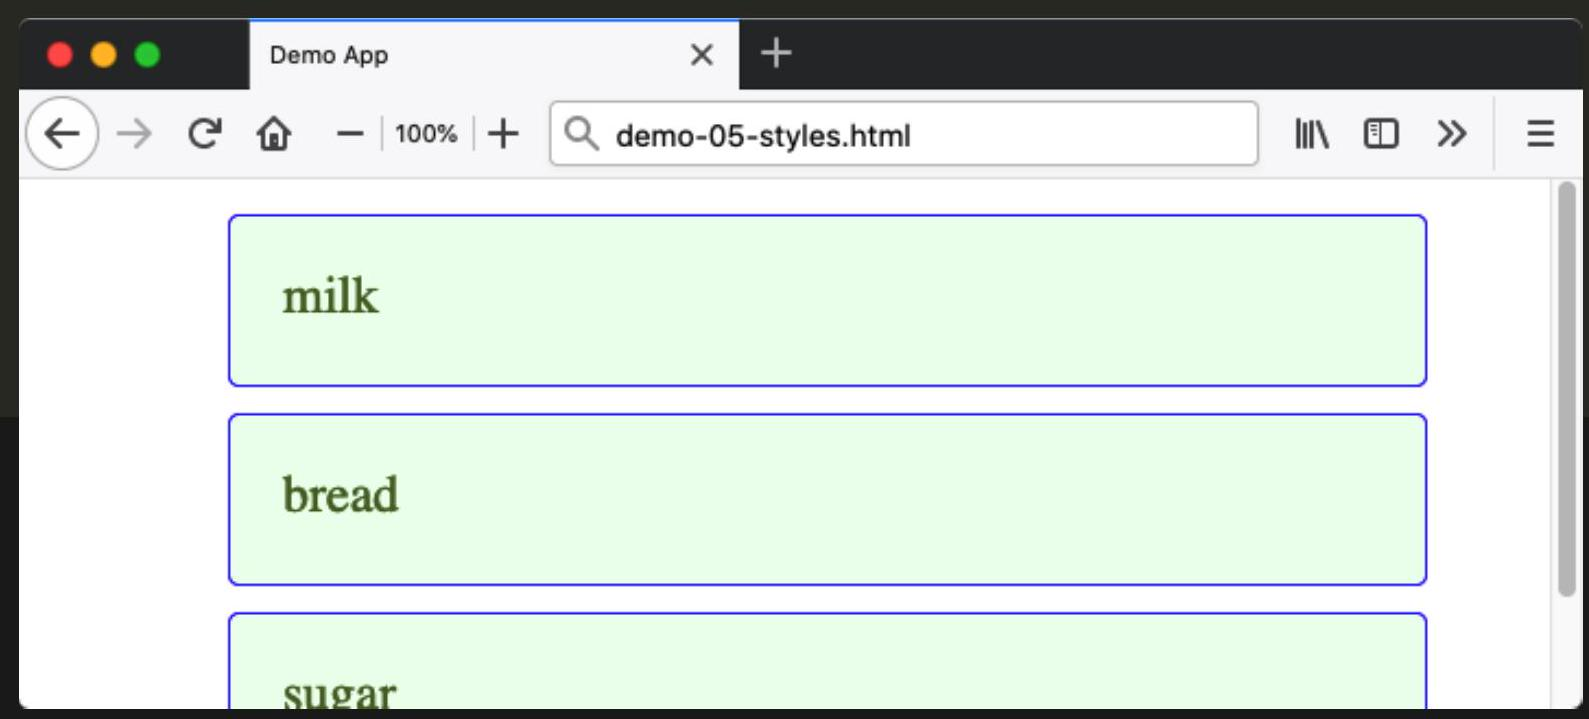
\includegraphics[width=\linewidth]{images/2025_01_02_254b5e4c52d090c313e1g-35}
  \end{center}
  
  \section*{ÜBERSICHT}
  \begin{itemize}
    \item Interne Repräsentation und das DOM
    \item Komponenten und Properties
    \item Darstellung von Komponenten
    \item Defaults und weitere Beispiele
  \end{itemize}
  
  \section*{DEFAULT PROPERTIES}
  \begin{verbatim}
  const App = () => (
          ["main",
              [MyButton, {disabled: true, text: 'Delete'}],
              [MyButton] ]
  )
  const MyButton = ({disabled=false, text='Button'}) => (
      ["button", disabled ? {disabled} : {}, text]
  )
  \end{verbatim}
  
  demo-09-defaultprops
  
  \section*{DEFAULT PROPERTIES}
  \begin{itemize}
    \item Übergebene Properties überschreiben Defaults
    \item Selbst zu implementieren (ist einfach, s. Beispiel)
    \item In React.js können Defaults an Funktion gehängt werden: (in SuiWeb nicht umgesetzt, wäre aber möglich)
  \end{itemize}
  
  \begin{verbatim}
  const MyButton = (props) => { ... }
  MyButton.defaultProps = {
      text: 'My Button',
      disabled: false,
  }
  \end{verbatim}
  
  \section*{WEITERES BEISPIEL}
  \begin{verbatim}
  const MyButton = ({children, disabled=true}) =>
      ["button", {style: "background: khaki", disabled}, ...children]
  const Header = ({name, children}) =>
      ["h2", "Hello ", name, ...children]
  const App = (props) =>
      ["div",
          [Header, {name: props.name}, " and", ["br"], "web developers"],
          [MyButton, "Start", {disabled:false}],
          [MyButton, "Stop"] ]
  useSJDON(App, Header, MyButton)
  render([App, {name: "SuiWeb"}], container)
  \end{verbatim}
  
  demo-10-children
  
  \section*{ZAHLEN IN PROPS}
  \begin{verbatim}
  const App = ({num1, num2}) =>
      ["h1", num1, " * ", num2, " = ", num1*num2]
  const element = [App, {num1: 3, num2: 9}]
  \end{verbatim}
  
  \begin{itemize}
    \item Beim Funktionsaufruf als Zahlen behandelt
    \item Beim Rendern in Textknoten abgelegt\\
  demo-11-numbers\\
  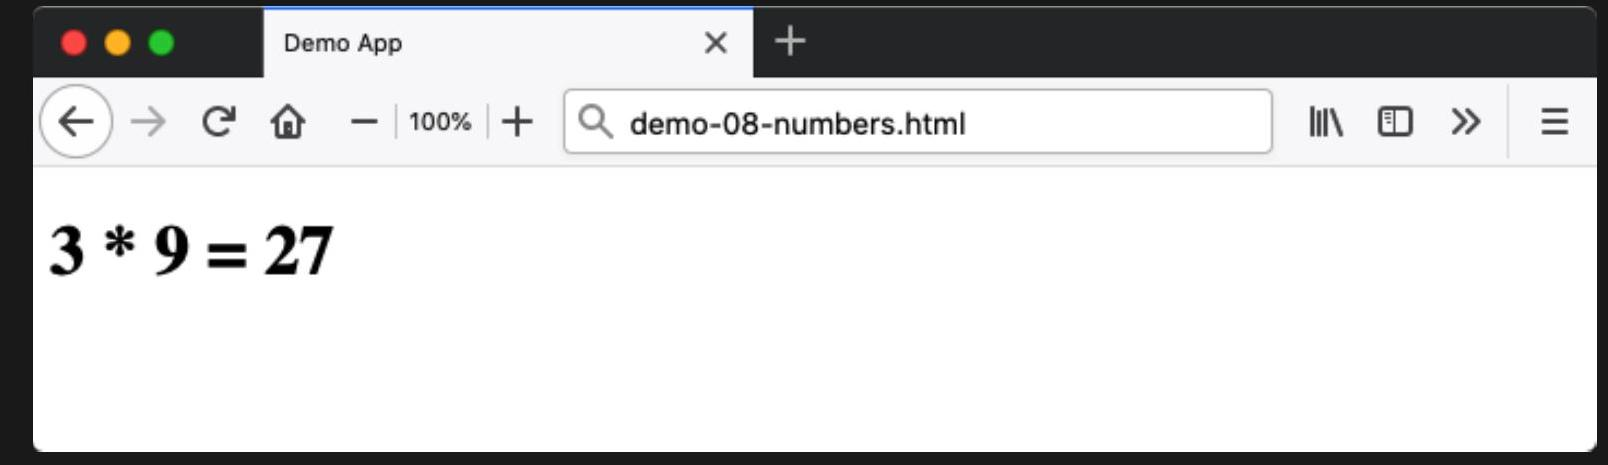
\includegraphics[width=\linewidth]{images/2025_01_02_254b5e4c52d090c313e1g-40}
  \end{itemize}
  
  \section*{AKTUELLER STAND}
  \begin{itemize}
    \item Notationen, um Komponenten zu definieren: JSX, SJDON
    \item Funktionen zur Anzeige im Browser: render-Funktion
    \item Daten können Komponenten steuern: Argument props
    \item Ausserdem: Verarbeiten von Styles, Default-Properties
    \item Also: Ul-Aufbau mit Komponenten
    \item Was noch fehlt: Mutation, Zustand\\
  $\rightarrow$ nächste Woche :)
  \end{itemize}

\subsection{UI Einsatz}

\section*{ÜBERSICHT}
\begin{itemize}
  \item Zustand von Komponenten
  \item Komponenten-Design
  \item Optimierungsansätze
\end{itemize}

\section*{ÜBERSICHT}
\begin{itemize}
  \item Zustand von Komponenten
  \item Komponenten-Design
  \item Optimierungsansätze
\end{itemize}

\section*{ZUSTAND}
\begin{itemize}
  \item Komponenten sollen auch einen Zustand haben können
  \item In React möglich, zum Beispiel mit als Klassen implementierten Komponenten
  \item Neuere Variante: Hooks, in diesem Fall: State-Hook
\end{itemize}

\section*{STATE-HOOK IN REACT}
const [stateVar, setStateVar] = useState(initialValue)

\begin{itemize}
  \item useState liefert Zustand und Update-Funktion
  \item Initialwert wird als Argument übergeben
  \item Zustandsänderung führt zum erneuten Rendern der Komponente
\end{itemize}

\section*{STATE-HOOK IN REACT}
\begin{verbatim}
const Counter = () => {
    const [state, setState] = useState(1)
    const handler = () => setState(c => c + 1)
    return (
        ["h1", {onclick:handler, style:{userSelect:"none",cursor:"pointer"}},
            "Count: " + state]
    )
}
const element = [Counter]
\end{verbatim}

\section*{STATE-HOOK: UMSETZUNG}
\begin{itemize}
  \item Aktuelles Element erhält ein Attribut hooks (Array)
  \item Beim Aufruf der Komponente wird useState aufgerufen
  \item Dabei: Hook angelegt mit altem Zustand oder Initialwert
  \item Ausserdem wird setstate definiert:
  \item Aufrufe in einer Queue im Hook speichern
  \item Re-render des Teilbaums anstossen
  \item Nächster Durchgang: alle Aktionen in Queue ausführen
\end{itemize}

\section*{STATE-HOOK IN SUIWEB}
\begin{itemize}
  \item State hooks sind auch in SuiWeb umgesetzt
  \item \href{https://suiweb.github.io/docs/tutorial/4-hooks}{https://suiweb.github.io/docs/tutorial/4-hooks}
\end{itemize}

\section*{BEISPIEL: EVENT}
\begin{verbatim}
import { render, useState, useSJDON } from "./lib/suiweb-1.1.js"
const Counter = () => {
    const [state, setState] = useState(1)
    const handler = () => setState(state + 1)
    return (
        ["h1", {onclick:handler, style:{userSelect:"none",cursor:"pointer"}},
            "Count: " + state]
    )
}
const element = [Counter]
\end{verbatim}

demo-21-state

\section*{BEISPIEL: TIMER (TEIL 1)}
\begin{verbatim}
const App = () => {
    let initialState = {
        heading: "Awesome SuiWeb (Busy)",
        content: "Loading...",
        timer: null,
    }
    let [state, setState] = useState(initialState)
    if (!state.timer) {
        setTimeout(() => {
            setState({ heading: 'Awesome SuiWeb', content: 'Done!',
            timer: true, })
        }, 3000)
    } ...
}
\end{verbatim}

\section*{BEISPIEL: TIMER (TEIL 2)}
\begin{verbatim}
const App = () => {
    const { heading, content } = state
    return ("
        ["main",
            [""h1", heading], ]
    )
}
\end{verbatim}

demo-22-state

\section*{BEISPIEL: TIMER}
\begin{itemize}
  \item Komponente zunächst mit Default-Zustand angezeigt
  \item Nach 3 Sekunden wird der Zustand aktualisiert
  \item Diese Änderung wird im UI nachgeführt
\end{itemize}

Das UI wird einmal deklarativ spezifiziert. Über die Zeit kann sich der Zustand der Komponente ändern. Um die Anpassung des DOM kümmert sich die Bibliothek.

\section*{BEISPIEL: ZÄHLER (TEIL 1)}
\begin{verbatim}
const Counter = (props) => {
    let [count, setCount] = useState(props.count)
    setTimeout(()=>setCount(count+1), 1000)
    return (
        ["p",
            {style: "font-size:2em"},
            "Count ", count ]
    )
}
\end{verbatim}

\section*{BEISPIEL: ZÄHLER (TEIL 2)}
\begin{verbatim}
const App = (props) =>
    ["div",
        [Counter, \{count: 1, key: 1\}],
        [Counter, \{count: 4, key: 2\}],
        [Counter, \{count: 7, key: 3\}] ]
\end{verbatim}

demo-23-state

\begin{center}
\begin{tabular}{|c|c|}
\hline
\multicolumn{2}{|l|}{-. Demapop $\times+$} \\
\hline
$\leftarrow \rightarrow \mathrm{C}$ ? - 1 100\% $++Q_{\text {demo-09-state.entm| }}$ & III  \\
\hline
Count 16 &  \\
\hline
Count 19 &  \\
\hline
Count 22 &  \\
\hline
\end{tabular}
\end{center}

\section*{ZUSTAND UND PROPERTIES}
\begin{itemize}
  \item Komponente kann einen Zustand haben (useState-Hook)
  \item Properties werden als Argument übergeben (props -Objekt)
  \item Zustand und Properties können Darstellung beeinflussen
  \item Weitergabe von Daten (aus Zustand und Properties) an untergeordnete Komponenten wiederum als Properties
\end{itemize}

\section*{KONTROLLIERTE EINGABE}
\begin{itemize}
  \item Zustand bestimmt, was in Eingabefeld angezeigt wird
  \item Jeder Tastendruck führt zu Zustandsänderung
  \item Problem: beim Re-Render geht der Fokus verloren
  \item In SuiWeb nur unbefriedigend gelöst: Index des Elements und Cursor-Position werden gespeichert
\end{itemize}

\section*{KONTROLLIERTE EINGABE}
\begin{verbatim}
const App = ({init}) => {
    let [text, setText] = useState(init)
    let [otherText, setOtherText] = useState("")
    const updateValue = e => {
        setText(e.target.value)
    }
    const updateOtherValue = e => {
        setOtherText(e.target.value)
    }
    return (
        ["div", {style: "background: lightblue"},
            ["h1", "Controlled Input Elements"],
            ["input", {oninput: updateValue, value: text}],
            ["p", "Your input: ", text ],
            ["textarea", {oninput: updateOtherValue}, otherText],
            ["p", "Your input: ", otherText ] ] )
}
const element = [App, {init: "Name"}]
demo-24-input
\end{verbatim}

\begin{center}
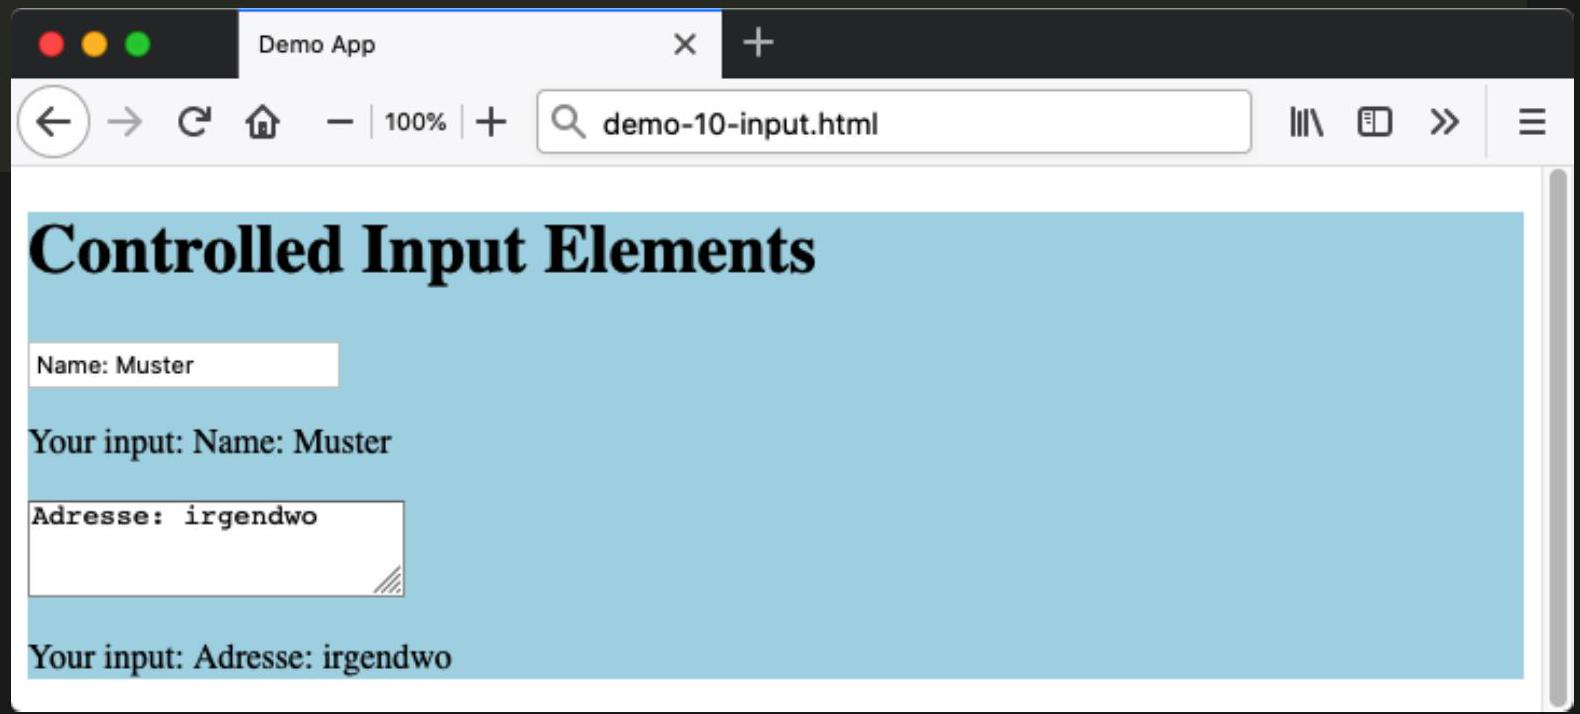
\includegraphics[width=\linewidth]{images/2025_01_02_a730400f36f38fd94791g-17}
\end{center}

\section*{KONTROLLIERTE EINGABE}
\begin{itemize}
  \item Ermöglicht es, nur bestimmte Eingaben zu erlauben
  \item Beispiel: nur Ziffern und Dezimalpunkt erlaubt
\end{itemize}

\begin{verbatim}
const updateValue = e => {
    const inp = e.target.value
    const reg = /^\d+\.?\d*$/
    if (reg.test(inp)) setText(inp)
    else setText(text)
}
\end{verbatim}

\section*{ÜBERSICHT}
\begin{itemize}
  \item Zustand von Komponenten
  \item Komponenten-Design
  \item Optimierungsansätze
\end{itemize}

\section*{CONTAINER-KOMPONENTE}
\begin{itemize}
  \item Daten-Verwaltung von Daten-Darstellung trennen
  \item Container-Komponente zuständig, Daten zu holen
  \item Daten per props an Render-Komponenten weitergegeben
  \item Übliches Muster in React-Applikationen
\end{itemize}

\section*{BEISPIEL}
\begin{verbatim}
/* Utility function that's intended to mock a service that this
/* component uses to fetch it's data. It returns a promise, just
/* like a real async API call would. In this case, the data is
/* resolved after a 2 second delay. */
function fetchData() {
    return new Promise((resolve) => {
            setTimeout(() => {
            resolve([ 'First', 'Second', 'Third' ])
        }, 2000)
        })
}
\end{verbatim}

5

\section*{CONTAINER-KOMPONENTE}
\begin{verbatim}
const MyContainer = () => {
    let initialState = { items: ["Fetching data..."] }
    let [state, setState] = useState(initialState)
    if (state === initialState) {
        fetchData()
            .then(items => setState(() => ({ items })))
    }
    return (
        [MyList, state]
    )
}
\end{verbatim}

demo-25-container

\section*{EFFECT HOOK}
\begin{itemize}
  \item Container-Komponenten haben verschiedene Aufgaben
  \item Zum Beispiel: Timer starten, Daten übers Netz laden
  \item In React unterstützen Klassen-Komponenten zu diesem Zweck verschiedene Lifecycle-Methoden, u.a.:\\
componentDidMount: Komponente wurde gerendert componentWillUnmount: Komponente wird gleich entfernt
  \item In Funktionskomponenten: Effect Hooks
  \item Funktionen, die nach dem Rendern ausgeführt werden\\
\href{https://react.dev/learn/synchronizing-with-effects}{https://react.dev/learn/synchronizing-with-effects}
\end{itemize}

\section*{EFFECT HOOK}
\begin{verbatim}
const MyContainer = () => {
    // after the component has been rendered, fetch data
    useEffect(() => {
        fetchData()
            .then(items => setState(() => ({ items })))
    }, []) ...
}
\end{verbatim}

\begin{itemize}
  \item React.js-Beispiel
  \item Hier ist ein weiteres Beispiel:\\
\href{https://suiweb.github.io/docs/tutorial/4-hooks#indexjs}{https://suiweb.github.io/docs/tutorial/4-hooks\#indexjs}
\end{itemize}

\section*{MONOLITHISCHE KOMPONENTEN}
\begin{itemize}
  \item Design-Entscheidung: wie viel UI-Logik in einer Komponente?
  \item Einfaches UI in einer einzelnen Komponente realisieren?
  \item Damit: weniger Komponenten zu entwickeln und pflegen
  \item Und: weniger Kommunikation zwischen Komponenten
\end{itemize}

\section*{Aber:}
\begin{itemize}
  \item Wenig änderungsfreundlich
  \item Kaum Wiederverwendung von Komponenten
\end{itemize}

\section*{BEISPIEL-ANWENDUNG}


\begin{itemize}
  \item Artikel können hinzugefügt werden
  \item Artikel: Titel, Zusammenfassung
  \item Klick auf den Titel: Inhalt einund ausblenden
  \item Klick auf X: Artikel löschen
\end{itemize}

\section*{AUFTEILUNG IN KOMPONENTEN}
\section*{Articles}
\begin{itemize}
  \item Article $1 \underline{x}$
\end{itemize}

Article 1 Summary

\begin{itemize}
  \item Article $2 \underline{X}$
  \item Article 3 X
  \item Article 4 X
\end{itemize}

\section*{ArticleList}
\section*{Articleltem}
\section*{AUFTEILUNG IN KOMPONENTEN}
\begin{verbatim}
const App = () => {
let initialState = { ...}
let [state, setState] = useState(...)
const onChangeTitle = e => { ... }
const onChangeSummary = e => { ... }
const onClickAdd = e => { ... }
const onClickRemove = (id) => { ... }
const onClickToggle = (id) => { ... }
\end{verbatim}

\begin{verbatim}
    return
    ["section",
        [AddArticle, {
            name: "Articles",
            title: state.title,
            summary: state.summary,
            onChangeTitle,
            onChangeSummary,
            onClickAdd,
        }],
    [ArticleList, {
        articles: state.articles,
        onClickToggle,
        onClickRemove,
    }] ]
)
}
\end{verbatim}

\section*{AUFTEILUNG IN KOMPONENTEN}
\begin{itemize}
  \item Komponente App kümmert sich um den Zustand
  \item Sie enthält: Event Handler zum Anpassen des Zustands
  \item Ausgabe übernehmen AddArticle und ArticleList
  \item Diese bekommen dazu den Zustand und die Handler in Form von Properties übergeben
\end{itemize}

\section*{APPLIKATIONSZUSTAND}
\begin{verbatim}
const App = () => {
    let initialState = {
        articles: [
            {
                id: cuid(),
                title: 'Article 1',
                summary: 'Article 1 Summary',
                display: 'none',
            },
            •••
        ],
        title: '',
        summary: '',
    }
}
\end{verbatim}

\section*{],}
\begin{verbatim}
title:
summary: ',
\end{verbatim}

\begin{itemize}
  \item Array von Artikeln
  \item Generierte IDs
  \item title und summary für Eingabefelder (controlled input)
\end{itemize}

\section*{EREIGNISBEHANDLUNG}
\begin{verbatim}
const App = () => {
    let initialState = { ...}
    let [state, setState] = useState(initialState)
    const onChangeTitle = e => {
        setState({...state, title: e.target.value})
    }
    const onClickRemove = (id) => {
        let articles = state.articles.filter(a => a.id != id)
        setState({...state, articles})
    }
    /*...*/
    return (...)
}
\end{verbatim}

\section*{AUFTEILUNG IN KOMPONENTEN}
\begin{verbatim}
const AddArticle = ({name, title, summary,
    onChangeTitle, onChangeSummary, onClickAdd}) => (
    ["section",
        ["h1", name],
        ["input", { placeholder: "Title", value: title,
                oninput: onChangeTitle }],
    ["input", { placeholder: "Summary", value: summary,
            oninput: onChangeSummary }],
    ["button", { onclick: onClickAdd }, "Add"] ]
)
\end{verbatim}

\section*{AUFTEILUNG IN KOMPONENTEN}
\begin{verbatim}
const ArticleList = ({articles, onClickToggle, onClickRemove}) => (
    ["ul", ...articles.map(i => (
        [ArticleItem, {
            key: i.id,
            article: i,
            onClickToggle,
            onClickRemove} ]))]
)
\end{verbatim}

demo-26-design

\section*{AUFTEILUNG IN KOMPONENTEN}
\begin{itemize}
  \item Zustand in wenigen Komponenten konzentriert
  \item Andere Komponenten für den Aufbau des UI zuständig
  \item Im Beispiel: Zustandsobjekt enthält kompletten Applikationszustand (inkl. Inhalt der Eingabefelder)
  \item Event Handler passen diesen Zustand an und basteln nicht am DOM herum
\end{itemize}

\section*{MODULE}
\begin{itemize}
  \item Komponenten können in eigene Module ausgelagert werden
  \item Zusammen mit komponentenspezifischen Styles
  \item Sowie mit lokalen Hilfsfunktionen
\end{itemize}

\section*{Separation of Concerns}
\begin{itemize}
  \item Wo sollte getrennt werden?
  \item Zwischen Markup und Styles und Programmlogik?
  \item Zwischen Komponenten?
\end{itemize}

\section*{MODULE}
\begin{verbatim}
import { ArticleItem } from "./ArticleItem.js"
const ArticleList = ({articles, onClickToggle, onClickRemove}) => (
    ["ul", ...articles.map(i => (
        [ArticleItem, {
            key: i.id,
            article: i,
            onClickToggle,
            onClickRemove} ]))]
)
export { ArticleList }
\end{verbatim}

demo-27-modules

\section*{NETZWERKZUGRIFF}
\begin{itemize}
  \item Letztes Beispiel erweitert
  \item Falls Artikelliste leer: Button zum Laden vom Netz
  \item Dazu stellt unser Express-REST-Service unter der id articles eine Artikelliste mit ein paar Mustereinträgen zur Verfügung
\end{itemize}

\section*{NETZWERKZUGRIFF}
\begin{verbatim}
const App = () => {
    let [state, setState] = useState(initialState)
    /* ... */
    return (
        ["section",
            [AddArticle, { ... } ],
            state.articles.length != 0
            ? [ArticleList, {articles: state.articles, onClickToggle, onClickRemove}]
            : ["p", ["button", {onclick: onLoadData}, "Load Articles"]]
        ]
    )
}
\end{verbatim}

\section*{NETZWERKZUGRIFF}
\begin{verbatim}
// Load articles from server
const onLoadData = () => {
    let url = 'http://localhost:3000/'
    fetch(url + "api/data/articles?api-key=wbeweb", {
        method: 'GET',
    })
        .then(response => response.json())
    .then(articles => setState({...state, articles}))
    .catch(() => {alert("Network connection failed")})
}
\end{verbatim}

demo-28-network

\section*{IMPERATIVER ANSATZ}
Ergänze alle Code-Teile in denen die Artikelliste erweitert oder verkleinert wird wie folgt:

\begin{itemize}
  \item Wenn der letzte Artikel gelöscht wird, entferne <uıl></ul> und füge einen Button für den Netzwerkzugriff ein
  \item Wenn der erste Artikel eingefügt wird, entferne den Button und füge ein  mit dem ersten / ein
  \item usw.
\end{itemize}

\section*{DEKLARATIVER ANSATZ}
\begin{itemize}
  \item Wenn die Artikelliste leer ist, wird ein Button ausgegeben
  \item Ansonsten wird die Artikelliste ausgegeben
\end{itemize}

Wir ändern nur den Zustand...

\section*{HAUPTKONZEPTE}
\begin{itemize}
  \item Klarer und einfacher Datenfluss:
  \item Daten nach unten weitergegeben (props)
  \item Ereignisse nach oben weitergegeben und dort behandelt
  \item Properties werden nicht geändert, Zustand ist veränderbar
  \item Zustand wird von Komponente verwaltet
  \item Es ist von Vorteil, die meisten Komponenten zustandslos zu konzipieren
\end{itemize}

\section*{ÜBERSICHT}
\begin{itemize}
  \item Zustand von Komponenten
  \item Komponenten-Design
  \item Optimierungsansätze
\end{itemize}

\section*{OPTIMIERUNGSANSÄTZE}
\begin{itemize}
  \item SuiWeb ist nicht für den produktiven Einsatz gedacht
  \item Im Folgenden werden Optimierungsansätze beschrieben
  \item Diese sind in SuiWeb nur teilweise implementiert
  \item Angelehnt an:
\end{itemize}

\begin{verbatim}
Rodrigo Pombo: Build your own React
https://pomb.us/build-your-own-react/
Zachary Lee: Build Your Own React.js in 400 Lines of Code
https://webdeveloper.beehiiv.com/p/build-react-400-lines-code
\end{verbatim}

Die Optimierungen werden hier nur grob skizziert und gehören nicht zum WBE-Pflichtstoff. Bei Interesse bitte angegebene Quellen konsultieren.

\section*{OPTIMIERUNG}
\section*{Problem:}
Die render-Funktion blockiert den Browser, was besonders beim Rendern grösserer Baumstrukturen problematisch ist

\section*{Abhilfe:}
\begin{itemize}
  \item Zerlegen der Aufgabe in Teilaufgaben
  \item Aufruf mittels requestIdleCallback
  \item Achtung: experimentelle Technologie
  \item React selbst verwendet dafür mittlerweile ein eigenes Paket „FWIW we've since stopped using requestIdleCallback..." \href{https://github.com/facebook/react/issues/11171}{https://github.com/facebook/react/issues/11171}
\end{itemize}

\section*{OPTIMIERUNG}
\begin{verbatim}
let nextUnitOfWork = null
function workLoop (deadline) {
    let shouldYield = false
    while (nextUnitOfWork && !shouldYield) {
        nextUnitOfWork = performUnitOfWork(
            nextUnitOfWork
        )
        shouldYield = deadline.timeRemaining() < 1
    }
    requestIdleCallback(workLoop)
}
requestIdleCallback(workLoop)
function performUnitOfWork (nextUnitOfWork) {
    // TODO
}
\end{verbatim}

\section*{OPTIMIERUNG: FIBERS}
\begin{itemize}
  \item Offen: wie wird das Rendern in Teilaufgaben zerlegt?
  \item Datenstruktur: Fiber Tree
  \item Ziel: einfaches Auffinden des nächsten Arbeitsschritts
  \item Fiber heisst eigentlich Faser
  \item Terminologie hier: Arbeitspaket (eigentlich: Unter-/Teilauftrag)
\end{itemize}

\section*{FIBERS: DATENSTRUKTUR}
[div, [h1, p, a], h2]

\begin{itemize}
  \item Elemente geeignet verlinkt
  \item Jedes Arbeitspaket kennt
  \item erstes Kind (first child)
  \item nächstes Geschwister (next sibling)
  \item übergeordnetes Element (parent)
\end{itemize}

\section*{FIBERS: NÄCHSTER SCHRITT}
\begin{itemize}
  \item Kind falls vorhanden
  \item sonst: nächstes Geschwister falls vorhanden
  \item sonst: Suche nach oben bis Element mit Geschwister
  \item sonst: fertig
\end{itemize}

\section*{FIBERS: IMPLEMENTIERUNG}
\begin{itemize}
  \item Funktion render aufgeteilt
  \item Legt nun erstes Arbeitspaket fest
  \item In createDom wird DOM-Knoten mit Attributen angelegt
\end{itemize}

\begin{verbatim}
let nextUnitOfWork = nul1
function render (element, container) {
    // erstes Arbeitspaket festlegen
}
function workLoop (deadline) {
    // Arbeitspakete bearbeiten
}
\end{verbatim}

\section*{FIBERS: IMPLEMENTIERUNG}
\begin{itemize}
  \item Noch offen: performUnitOfWork
  \item Bearbeitet aktuellen Auftrag und liefert nächsten Auftrag
  \item Dieser wird im while gleich bearbeitet, falls Browser idle
  \item Sonst im nächsten requestIdleCall.back
\end{itemize}

\begin{verbatim}
function performUnitOfWork (fiber) {
    // TODO add dom node
    // TODO create new fibers
    // TODO return next unit of work
}
\end{verbatim}

\section*{FIBERS: IMPLEMENTIERUNG}
\begin{verbatim}
function performUnitOfWork(fiber) {
    // TODO add dom node
    // TODO create new fibers
    // TODO return next unit of work
}
\end{verbatim}

\begin{itemize}
  \item Knoten anlegen ( createDom) und ins DOM einhängen
  \item Für jedes Kindelement Arbeitspaket (Fiber) anlegen
  \item Referenzen eintragen (sibling, parent, child)
  \item Nächstes Arbeitspaket suchen und zurückgeben
\end{itemize}

\section*{AUFTEILUNG IN ZWEI PHASEN}
\section*{Erste Phase:}
\begin{itemize}
  \item Fibers anlegen
  \item DOM-Knoten anlegen (dom-Attribut)
  \item Properties hinzufügen
  \item Fibers verlinken: parent, child, sibling
\end{itemize}

\section*{Zweite Phase:}
\begin{itemize}
  \item DOM-Teil der Fibers (. .dom ) ins DOM hängen
\end{itemize}

Implementierung: s. Step V: Render and Commit Phases\\
\href{https://pomb.us/build-your-own-react/}{https://pomb.us/build-your-own-react/}

\section*{ABGLEICH MIT LETZTER VERSION}
\begin{itemize}
  \item Ziel: nur Änderungen im DOM nachführen
  \item Referenz auf letzte Version des Fiber Tree: currentRoot
  \item Jedes Fiber erhält Referenz auf letzte Version: alternate
  \item Nach der Aktualisierung wird aktuelle zur letzten Version
  \item Unterscheidung von update - und placement -Fibers
  \item Ausserdem eine Liste der zu löschenden Knoten
\end{itemize}